\hypertarget{introduction}{%
\section{Introduction}\label{introduction}}

\hypertarget{informations-utiles}{%
\subsection{Informations utiles}\label{informations-utiles}}

\hypertarget{professeurs}{%
\subsubsection{Professeurs}\label{professeurs}}

\begin{itemize}
\tightlist
\item
  HAMRI Maamar El Amine,
  \href{mailto:amine.hamri@univ-amu.fr}{\nolinkurl{amine.hamri@univ-amu.fr}}
\item
  MASSAT Jean luc,
  \href{mailto:jean-luc.massat@univ-amu.fr}{\nolinkurl{jean-luc.massat@univ-amu.fr}}
\item
  YACOUB Aznam, pas de mail donné
\end{itemize}

\hypertarget{volume-horaire}{%
\subsubsection{Volume horaire}\label{volume-horaire}}

\begin{itemize}
\tightlist
\item
  9 cours de 2h
\item
  9 TD de 2h
\item
  9 TP de 2h
\end{itemize}

\hypertarget{modalituxe9s-de-contruxf4le-des-connaissances}{%
\subsubsection{Modalités de contrôle des
connaissances}\label{modalituxe9s-de-contruxf4le-des-connaissances}}

Première session: \(NoteFinale = 0.6 * ExamenTerminal + 0.4 * Projet\)

Avec \(Proj = \max(0.3 * Projet1 + 0.7 * Projet2, Projet2)\)

L'examen terminal sera en décembre et durera 3H. Les documents ne seront
pas autorisés.

Les deux projets se dérouleront sur environ 3 et 7 semaines.

\hypertarget{projets}{%
\subsubsection{Projets}\label{projets}}

Les projets sont de taille conséquente, il est donc conseillé de former
des équipes de 5. Les changements d'équipe seront impossible après le
début des projets.

Il est à priori possible de se mettre en équipe avec des étudiants
d'autres groupes, mais à condition que l'EDT soit bon (il faudra
demander au professeur).

\hypertarget{pruxe9sentation-guxe9nuxe9rale}{%
\subsection{Présentation
générale}\label{pruxe9sentation-guxe9nuxe9rale}}

\textbf{NOTE} : regarder le poly sur ametice sera surement plus
représentatif du cours, l'intégralité du contenu est (sera) dessus.

Le génie logiciel étudie des méthode et outils qui permettent de
déveloper des logiciels de taille conséquente en gardant une qualité
élevée, et une maitrise des coûts de developpement et des délais. Cette
science ne se concentre pas sur le code, mais sur des solutions qui vont
faciliter l'implémentation.

\hypertarget{plan-du-cours}{%
\subsubsection{Plan du cours}\label{plan-du-cours}}

\begin{itemize}
\tightlist
\item
  Intéret d'adopter un cycle de vie
\item
  Présentation d'une méthode de developpement logiciel
\item
  Présenter comment coder, organiser le code, intérêt des test, \ldots{}
\end{itemize}

\hypertarget{constat}{%
\subsubsection{Constat}\label{constat}}

Pour beaucoup de projets informatiques :

\begin{itemize}
\tightlist
\item
  le produit ne répond pas au cahier des charges.
\item
  le produit est livré hors délai.
\item
  lors de la maintenance, des erreurs se manifestent à cause d'une
  mauvaise hygiène de code.
\end{itemize}

L'objectif est de construire des logiciels ergonomiques, fiables,
évolutifs \& économiquement viables.

\hypertarget{indicateurs-utiles-sur-un-projet}{%
\subsubsection{Indicateurs utiles sur un
projet}\label{indicateurs-utiles-sur-un-projet}}

\begin{itemize}
\tightlist
\item
  \emph{Volume} : le nombre d'instruction (en KLS : Kilo Lignes Sources)
\item
  \emph{Effort} : le temps nécessaire pour un ingénieur (en HA :
  \href{https://fr.wiktionary.org/wiki/homme-ann\%C3\%A9e}{Hommes
  Années})
\item
  \emph{Délai de réalisation}
\item
  \emph{Durée de vie} : le temps pendant lequel le logiciel devra être
  maintenu
\end{itemize}

\hypertarget{la-qualituxe9-logicielle}{%
\subsubsection{La qualité logicielle}\label{la-qualituxe9-logicielle}}

Un logiciel peut être observé selon ses qualités, qui sont :

\begin{itemize}
\tightlist
\item
  soit internes, comme la modularité, la maintenabilité, \ldots{}
\item
  soit externes, comme la validité, la robustesse, la performance,
  \ldots{}
\end{itemize}

Durant le développement, on va principalement voir les qualités
internes.

Les facteurs de qualité ne sont pas nécessairement compatibles 2 à 2, il
faut souvent trouver un compromis.

\hypertarget{duxe9finitions}{%
\subsection{Définitions}\label{duxe9finitions}}

Une méthode est un semble de règles qui consuisent à une solution.

Une méthodologie est une agrégation de méthodes, guides, outils,
techniques de différents domaines permettant de déduire la manière de
résoudre un problème.

La modélisation est une activité qui précède toute décision ou
formulation.

Un modèle est une interprétation de la compréhenstion d'une situation ou
d'une idée de la situation.

\hypertarget{moduxe8le-de-duxe9veloppement-le-cycle-de-vie}{%
\subsection{Modèle de développement : le cycle de
vie}\label{moduxe8le-de-duxe9veloppement-le-cycle-de-vie}}

\href{https://fr.wikipedia.org/wiki/Cycle_de_d\%C3\%A9veloppement_(logiciel)}{Cliquer pour voir
l'article sur wikipedia}

La gestion de projet nécessite la modélisation du processus de
developpement lui-mème. C'est ce à quoi le cycle de vie sert.

Il faut savoir que ce modèle n'est pas unique, et que d'autres modèles
existent comme par exemple la méthode agile, ou la méthode merise. Ces
méthodes peuvent être plus adaptées à certains types de logiciels.

Plusieurs modèles de cycle de vie ont été élaborés. Tous ont en commun
au minimum les 5 phases essentielles de tout développement :

\begin{itemize}
\tightlist
\item
  la spécification (cahier des charges)
\item
  la conception
\item
  la réalisation
\item
  les test
\item
  l'exploitation
\end{itemize}

\hypertarget{le-moduxe8le-de-la-cascade}{%
\subsubsection{Le modèle de la
cascade}\label{le-moduxe8le-de-la-cascade}}

Ce modèle est inspiré de l'industrie du batiment, et repose sur les
principes suivants :

\begin{itemize}
\tightlist
\item
  on ne peut pas construire la toiture avant les fondations
\item
  les conséquences d'une modification en amont du cycle ont un impact
  majeur sur les coûts en aval
\end{itemize}

Ainsi, dans ce modèle, les taches sont executées séquentiellement, et en
conséquent les erreurs sont détectées tardivement (lors de la livraison
du produit) et le processus pour les fixer sera donc long et coûteux.

\href{https://fr.wikipedia.org/wiki/Cycle_de_d\%C3\%A9veloppement_(logiciel)\#/media/Fichier:Mod\%C3\%A8le_en_cascde.svg}{\begin{center}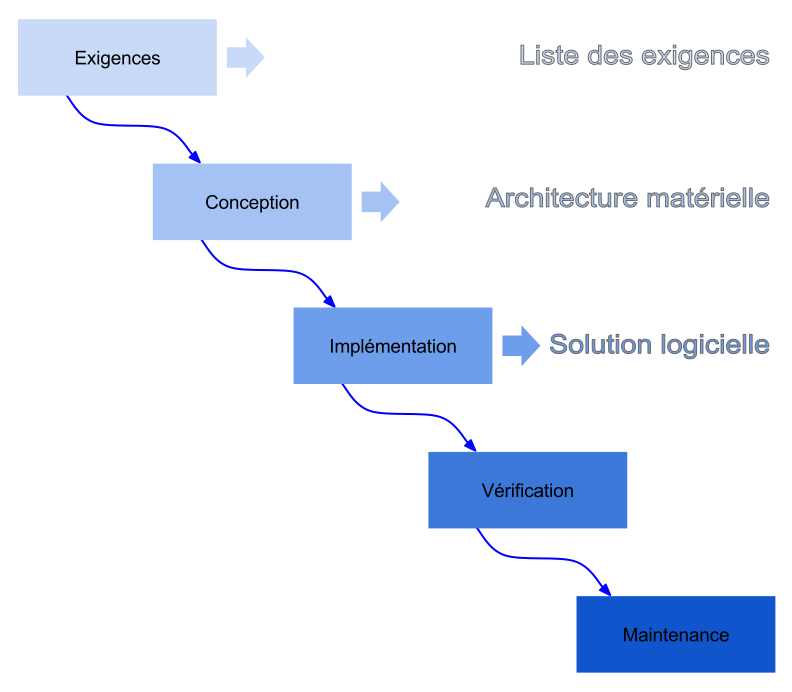
\includegraphics[width=0.8\textwidth]{assets/cascade.png}\end{center}}

\hypertarget{le-moduxe8le-en-v}{%
\subsubsection{Le modèle en V}\label{le-moduxe8le-en-v}}

Ce modèle, qui est encore aujourd'hui très utilisé, a été proposé pour
combler les lacunes du modèle en cascade, c'est à dire (principalement)
la tardiveté de la détection des erreurs.

Pour cela, il définit des tests qui permettent de tester les composants
indépendaments. en effet, chaque phase de développement est associée
avec la phase de validation qui lui correspond.

\href{https://fr.wikipedia.org/wiki/Cycle_de_d\%C3\%A9veloppement_(logiciel)\#/media/Fichier:Cycle_de_developpement_en_v.svg}{\begin{center}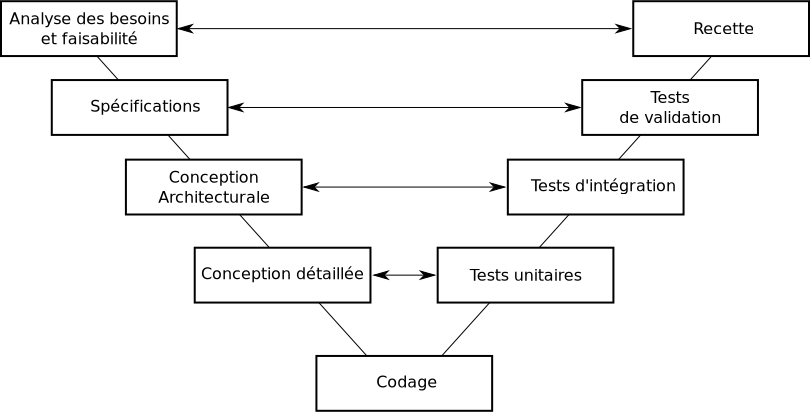
\includegraphics[width=0.8\textwidth]{assets/v.png}\end{center}}

Note : la ``recette'' correspond à des test d'acceptation.

Note : C'est le modèle que l'on va adopter pour le premier projet.

\hypertarget{le-moduxe8le-en-spirale}{%
\subsubsection{Le modèle en spirale}\label{le-moduxe8le-en-spirale}}

Cette méthode reprend les différentes étapes du cycle en V. Elle est
liée aux projets innovants où il est difficile de cerner les besoins du
client.

Elle permet ainsi de pouvoir changer le cahier des charges plusieurs
fois, ce qui serait impossible avec un modèle en spirale.

\href{https://fr.wikipedia.org/wiki/Mod\%C3\%A8le_en_spirale\#/media/Fichier:Spirale_(Boehm,_1988).svg}{\begin{center}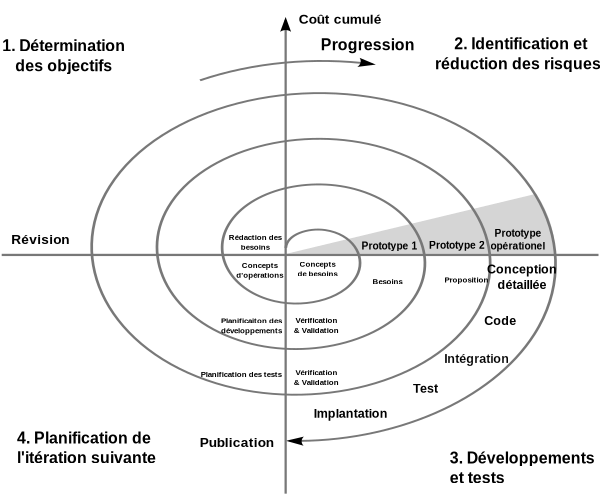
\includegraphics[width=0.8\textwidth]{assets/spirale.png}\end{center}}
